% For tracking purposes - this is V2.0 - May 2012

\documentclass{sig-alternate-05-2015}
\usepackage[vlined, ruled]{algorithm2e}
\usepackage{multirow}
\begin{document}

%\setcopyright{acmlicensed}

%Conference
\conferenceinfo{GECCO'17,} {July 15-19, 2017, Berlin, Germany}
\CopyrightYear{2017}
\crdata{TBA}
\clubpenalty=10000
\widowpenalty = 10000



\title{Two-edge Graphical Linkage Model for DSMGA-II}

\numberofauthors{2} 
\author{
% 1st. author
\alignauthor
Author\\
       \affaddr{Address}\\
       \affaddr{Address}\\
       \affaddr{Address}\\
       \email{email}
%Ping-Lin Chen\titlenote{These authors contributed equally to this work.}\\
%       \affaddr{Taiwan Evolutionary Intelligence Laboratory}\\
%       \affaddr{Department of Electrical Engineering}\\
%       \affaddr{National Taiwan University}\\
%       \email{r04921043@ntu.edu.tw}
%% 2nd. author
\alignauthor
Author\\
       \affaddr{Address}\\
       \affaddr{Address}\\
       \affaddr{Address}\\
       \email{email}
%\alignauthor
%Chun-Jen Peng\titlenote{These authors contributed equally to this work.}\\
%       \affaddr{Taiwan Evolutionary Intelligence Laboratory}\\
%       \affaddr{Department of Electrical Engineering}\\
%       \affaddr{National Taiwan University}\\
%       \email{r04921039@ntu.edu.tw}
\and  % use '\and' if you need 'another row' of author names
%% 3rd. author
\alignauthor
Author\\
       \affaddr{Address}\\
       \affaddr{Address}\\
       \affaddr{Address}\\
       \email{email}
%\alignauthor Chang-Yi Lu\\
%       \affaddr{Taiwan Evolutionary Intelligence Laboratory}\\
%       \affaddr{Department of Electrical Engineering}\\
%       \affaddr{National Taiwan University}\\
%       \email{r03921053@ntu.edu.tw}
%% 4th. author
\alignauthor
Author\\
       \affaddr{Address}\\
       \affaddr{Address}\\
       \affaddr{Address}\\
       \email{email}
%\alignauthor Tian-Li Yu\\
%       \affaddr{Taiwan Evolutionary Intelligence Laboratory}\\
%       \affaddr{Department of Electrical Engineering}\\
%       \affaddr{National Taiwan University}\\
%       \email{tianliyu@ntu.edu.tw}
}


\maketitle
\begin{abstract}
DSMGA-II, a model-based genetic algorithm, is capable of solving optimization problems via exploiting sub-structures of the problem. In terms of number of function evaluations (NFE), DSMGA-II has shown superior optimization ability to LT-GOMEA and hBOA on various benchmark problems as well as real-world problems. This paper proposes a two-edge graphical linkage model, which customizes recombination masks for each receiver according to its alleles, to further improve the performance of DSMGA-II.  The new linkage model is more expressive than the original dependency structure matrix (DSM), providing far more possible linkage combinations than the number of solutions in the search space. To reduce unnecessary function evaluations, the two-edge model is used along with the supply bounds from the original DSM. Some new techniques are also proposed to enhance the model selection efficiency and to reduce the probability of cross-competition. Combining these proposed techniques, the empirical results show up to 20\% of NFE reduction compared with the original DSMGA-II.
\end{abstract}


%
% The code below should be generated by the tool at
% http://dl.acm.org/ccs.cfm
% Please copy and paste the code instead of the example below. 
%
\begin{CCSXML}
<ccs2012>
<concept>
<concept_id>10010293.10010300.10010302</concept_id>
<concept_desc>Machine learning approaches~Maximum entropy modeling</concept_desc>
<concept_significance>500</concept_significance>
</concept>
<concept>
<concept_id>10010293.10011809.10011812</concept_id>
<concept_desc>Machine learning approaches~Genetic algorithms</concept_desc>
<concept_significance>500</concept_significance>
</concept>
<concept>
<concept_id>10010293.10010300.10010304</concept_id>
<concept_desc>Machine learning approaches~Mixture models</concept_desc>
<concept_significance>300</concept_significance>
</concept>
</ccs2012>
\end{CCSXML}

\ccsdesc[500]{Machine learning approaches~Maximum entropy modeling}
\ccsdesc[500]{Machine learning approaches~Genetic algorithms}
\ccsdesc[300]{Machine learning approaches~Mixture models}
%
% End generated code
%

%
%  Use this command to print the description
%
\printccsdesc

\keywords{Genetic Algorithm; Estimation-of-Distribution Algorithm; Linkage Learning; Model Building}

\section{Introduction}

Dependency structure matrix genetic algorithm-II (DSMGA-II) is a novel model building GA proposed by Hsu and Yu in 2015~\cite{hsu:DSMGA2}.
Based on the dependency structure matrix (DSM), a new linkage model, called the incremental linkage set (ILS), is adopted in DSMGA-II to provide potential models for mixing. The restricted mixing and back mixing are the two major recombination operators of DSMGA-II. They are the keys to significantly reduce the number of function evaluations (NFE) compared with other optimal mixing operators. Experiment results show that DSMGA-II requires fewer function evaluations  than  LT-GOMEA~\cite{bosman:LT-GOMEA} and hBOA~\cite{pelikan:hBOA}, two cutting-edge evolutionary algorithms, on various benchmark problems. 

However, there is still room for improvement with model building in DSMGA-II. In this paper, we consider building a two-edge graphical linkage model as a more effective linkage model. We also demonstrate how early-stopping methods enable more efficient model selection during mixing, resulting in less NFE.


This paper is organized in five parts. Section 2 introduces the original DSMGA-II schema. Section 3 introduces the two-edge linkage model in detail, along with some new techniques to enhance mixing effectiveness. Section 4 shows the experiment results. Section 5 gives the summary and conclusion.



\section{DSMGA-II}
In this section, we first introduce the framework of DSMGA-II and the concept of incremental linkage set. Then we give details of restricted mixing and back mixing, which are the kernel operators of DSMGA-II.

\begin{algorithm}
\caption{DSMGA-II}\label{algo_disjdecomp}
\SetKwData{Left}{left}\SetKwData{This}{this}\SetKwData{Up}{up}

\SetKwFunction{PopulationInitialization}{PopulationInitialization}
\SetKwFunction{GHC}{GHC}
\SetKwFunction{ShouldTerminate}{ShouldTerminate}
\SetKwFunction{TournamentSelection}{TournamentSelection}
\SetKwFunction{UpdateMatrix}{UpdateMatrix}
\SetKwFunction{RestrictedMixing}{RestrictedMixing}
\SetKwFunction{BackMixing}{BackMixing}

$P$: population, $S$: selected population, \\
$s$: selection pressure, $R$: constant, \\
$DSM$: dependency structure matrix, $M$: mask \\

\SetKwInOut{Input}{input}\SetKwInOut{Output}{output}
\Input{ $l$: problem size, $p$: population size }
\Output{ $P_{best}$ }

\BlankLine

$P \leftarrow$ \PopulationInitialization{$l$, $p$} \\
$P \leftarrow$ \GHC{$P$} \\
\While{not \ShouldTerminate}{
    $S \leftarrow$ \TournamentSelection{$P$, $s$} \\
    $DSM \leftarrow $ \UpdateMatrix{$S$} \\

    \For{$k\leftarrow 1$ \KwTo $R$}{
        $I \leftarrow$ random permutation from 1 to $p$ \\

        \For{$i \in I$}{
            $P_i$, $M \leftarrow$ \RestrictedMixing{$P_i$} \\
            \If{$M \neq \emptyset$} {
                $P \leftarrow$ \BackMixing{$P_i$, $M$} \\
            }
        }
    }
}
\Return best instance in $P$
\end{algorithm}


\subsection{Framework of DSMGA-II}
DSMGA-II consists of four major steps: population initialization, linkage model building, restricted mixing and back mixing. 

First, DSMGA-II randomly initializes a population. Then, in order to enhance the quality of pairwise linkage model and reduce the noise in the population, DSMGA-II performs a bit-flipping greedy hill climbing (GHC) on each chromosome. For each randomly initialized chromosome, GHC randomly flips each bit in the chromosome and evaluates its fitness. If the fitness improves, the chromosome accepts the change. Otherwise, the flipped bit is restored. Pairwise linkage detection was adopted in a later version of LTGA~\cite{pelikan:pairwise} and DSMGA~\cite{yu:DSMGA} due to its resistance to sampling noise. Performing GHC before linkage model building can further ensure the pairwise linkage information between genes, by ruling out trivial cases that can be solved without linkage information. 


After initializing the population, only the selected chromosomes are used to build the linkage model. The chromosomes are chosen by a tournament selection with selection pressure as 2, suggested in~\cite{yu:population}. DSMGA-II adopts mutual information as pairwise linkage measure and stores the linkage information in a DSM. The DSM is updated only once in each generation in order to prevent overfitting from frequent model building. Notice that tournament selection is only performed to choose chromosomes for model building instead of updating the population. The following steps of restricted mixing and back mixing proceed with the original population.


Before mixing, DSMGA-II builds the ILS with the linkage information stored in DSM. The ILS is a set of models indicating possible subproblem structures for restricted mixing. In restricted mixing, the receiver tries to flip the bits within the model. If the fitness does not decrease, the receiver becomes the donor in back mixing and the new pattern is tried on all chromosomes in the population. The population is randomly shuffled before restricted mixing so that each chromosome takes turns acting as the receiver in restricted mixing and the donor in back mixing. The pseudo code of DSMGA-II is given in Algorithm 1. The detailed implementations of the ILS and the mixing operators are described in the following sections. 



\subsection{Incremental Linkage Set}
The DSM is an adjacent matrix representing the dependency between two variables, where each entry stores the pairwise information between two bits. In DSMGA-II, pairwise dependencies are measured by mutual information~\cite{kullback:KL-diversion}. Formally, the mutual information of two random variable X and Y can be defined as:

\begin{displaymath} 
I(X;Y) = \sum_{x \in X}\sum_{y \in Y} p(x,y)  log \frac{p(x,y)}{p(x) p(y)}, 
\end{displaymath}
where x and y are the outcomes of X and Y. In pairwise information, the random variables X and Y follows the (binomial) Bernoulli distribution with support \{0, 1\}. p(x) represents the portion of a bit having value 1 in the population. Therefore, the linkage measure can be further derived as:

\begin{equation} 
\begin{split}
I(X;Y) &= P_{00 }log\frac{P_{00}}{P_{0*} P_{*0}} + P_{11 }log\frac{P_{11}}{P_{1*} P_{*1}}  \\
	    &+ P_{01 }log\frac{P_{01}}{P_{0*} P_{*1}} + P_{10 }log\frac{P_{10}}{P_{1*} P_{*0}}  
\end{split}
\end{equation}


If X and Y are independent, then I(X; Y) equals to 0.
Otherwise, the mutual information indicates how much the corresponding bits differ from most of the chromosomes in current population.
The value of mutual information between two bits corresponds to the probability of two bits being in the same building-block.
Therefore, DSMGA-II constructs building-blocks by clustering the DSM.
Instead of using traditional hierarchical clustering algorithms proposed in~\cite{thierens:LTGA} or the average linkage clustering technique proposed in~\cite{thierens:OM}, DSMGA-II adopts a specific subgraph called approximation maximum-weight connected subgraph (AMWCS).
DSMGA-II constructs AMWCS from a certain bit,  and iteratively adds one single bit into the graph.
%For example, consider a  graph $G = (V, E), V = \{v1 ,v2, v3, v4\}$, the AMWCS $G_{s} =(V_{s}, E_{s}), V_{s} =\{v1 , v2\}$, and the candidate nodes $N =\{v3 ,v4\}$. The goal is to find a node from the candidate set with a greedy approach that maximizes the weight of AMWCS after insertion. The equation can be defined as : 

%\begin{equation} \textit{index} = argmax_{i\in 3,4}\sum_{j=1}^{2} I(v_i;v_j) \end{equation}

%The ILS  is an AMWCS constructed with a randomly chosen start node. For example, consider a problem with problem size  4, and its linkage model, i.e. the DSM, shown in Figure 1. The first step of constructing ILS is to choose a start node. Here, the index 1 was randomly chosen from $\{1, 2, 3, 4\}$. Then, the rest of nodes are inserted into AMWCS following the sequence $\{1,2,4,3\}$ that gives the maximum weight. After 3 iterations, the ILS is constructed as an ordered set $L = \langle\{1\}, \{1, 2\}, \{1, 2, 4\}, \{1, 2, 4, 3\} \rangle$. Each component of the ILS is called a mask, which is a potential  building-block in the mixing stage. 




\subsection{Restricted Mixing and Back Mixing}

\subsubsection{Optimal Mixing}
Unlike canonical genetic algorithms that generate offsprings by recombining parental solutions, DSMGA-II extends the the idea of optimal mixing (OM)~\cite{thierens:OM} with two new mixing operators: restricted mixing and back mixing. OM evaluates a chromosome during recombination. With the information of fitness before and after mixing, the chromosome only accepts the change if its fitness improves. Thus, a noise-free decision-making can be achieved with a much smaller population size~\cite{goldberg:buildingblock}. Given overlapping building blocks, OM is also capable of solving problems with overlapping structures efficiently, since it acts like building-block wise local search.


\subsubsection{Restricted Mixing}

In in each iteration of restricted mixing, a receiver is randomly picked from the population, and the building-blocks are provided by a mask which is chosen from the ILS. Each mask is a set of indices that indicates which bits should be flipped together during mixing operations. All masks in the ILS must go through a supply check to make sure that the complement pattern of the receiver exists in the population.  After supply check, the receiver starts with the smallest subset in the mask, and flips the bits within the subset. If the fitness does not decrease after recombination, the pattern is accepted and restricted mixing terminates. The receiver then becomes the donor of the new pattern for rest the population in back mixing. 


The idea behind restricted mixing is building-block supply~\cite{goldberg:buildingblock}. We believe all the optimal subsolution fragments should exist in the current population, which had been initialized with a sufficient population size. Therefore, given the correct building block with a proper receiver, restricted mixing conducts optimal mixing between the receiver and the chromosome with the complementary optimal pattern. The pseudo-code for  restricted mixing is provided in Algorithm 2.

\begin{algorithm}
\caption{Restricted Mixing}\label{algo_disjdecomp}

$V$: candidate vertices set, $V_S$: $AMWCS$ vertices set,  \\
$ILS$: incremental linkage set, $f$: evaluation function, \\
$P$: population, $l$: problem size, \\
$T$: trial solution, $M$: mask, \\
${R_M}$: pattern of $R$ extracted by $M$, \\
${R_M}'$: complement pattern of ${R_M}$

\SetKwInOut{Input}{input}\SetKwInOut{Output}{output}
\Input{ $R$: receiver }
\Output{ $R$: reciever, $M$: mask }

\BlankLine
%\tcp{ construct ILS }
$V \leftarrow \{ 1, 2, ..., l \}$ \\
%$V_S \leftarrow \{v$ | a random vertex $v \in V \}$ \\
$V_s \leftarrow$ a random vertex $v \in V$ \\
remove $v$ from $V$ \\

\While{$ |V| \geq l/2$} {

    $ILS \leftarrow ILS \cup V_{S}$ \\
    $V_S \leftarrow V_S$ $\cup$ \{ the nearest vertex $v \in V \}$ \\
    %add the nearest vertex $v \in V$ into $AMWCS$ \\
    
    remove $v$ from $V$ \\
}

\BlankLine
\For{$i \leftarrow 1$ \KwTo $|ILS|$} {

    $M \leftarrow ILS_i$ \\

    \If {${R_M}' \subset P$} {

        $T \leftarrow R$ \\
        $T_M \leftarrow {R_M}'$ \\

        \If {$f(T) \geq f(R)$ and $T \notin P$} {
            $R \leftarrow T$ \\
            \Return ($R$, $M$)
        }
    }
}
\Return ($R$, $\emptyset$) 
\end{algorithm}


\subsubsection{Back Mixing}

In back mixing, every chromosome in the population is mixed with the pattern accepted in restricted mixing. Chromosomes are set to accept the new pattern only with strict fitness improvement by default. However, if no chromosome fitness improves in the whole population, then the mixing which results in equal fitness is also allowed. The back mixing acceptance criterion is set differently from restricted mixing in order to tackle real-world problems with plateaus and basins. Many operators, such as the forced improvement~\cite{bosman:LT-GOMEA}, have been developed to deal with multiple equal-quality solutions. Strict mixing improvement criterion often causes numerous evaluations to jump out of the plateaus. On the other hand, allowing all chromosomes to accept the patterns with equal fitness results in a strong drifting effect. Back mixing handles the diversity issue with a default strict-improvement criterion. When no improvement occurs, it switches to the equal-acceptance criterion to reduce unnecessary evaluations on plateaus. The empirical experiment results suggest that back mixing is able to deal with both plateaus and diversity issues. The pseudo-code for  restricted mixing is provided in Algorithm 3. 

\begin{algorithm}
\caption{Back Mixing}\label{algo_disjdecomp}

$P$: population, $f$: evaluation function, \\
$T$: trial solution, $E$: set of candidate solutions 

\SetKwInOut{Input}{input}\SetKwInOut{Output}{output}
\Input{ $D$: donor, $M$: mask }
\Output{ $P$: population }

\BlankLine

$improved  \leftarrow false$ \\
\For{$j \leftarrow 1$ \KwTo $|P|$} {

    $T \leftarrow P_j$ \\
    $T_M \leftarrow D_M$ \\

    \eIf {$f(T) \geq f(P_j)$} {

        $P_j \leftarrow T$ \\
        $improved  \leftarrow true$ \\
    }{
        \If {$f(T) = f(P_j)$} {
            $E \leftarrow E \cup \{T\}$ \\
        }
    }
}
\If {$not$ $improved$} {
    accept all solutions in $E$ \\
} 

\Return $P$

\end{algorithm} 





\section{THE TWO-EDGE GRAPHICAL LINKAGE MODEL}
This section introduces the concept and the flow of AMWCS construction. In the original AMWCS, nodes are connected with only one linkage. We call this technique the one-edge graphical linkage model. In this section, we first describe the new linkage graph, called the two-edge graphical linkage model, which gives customized building-block models for each chromosome. Then, we discuss \textit{supply bound}, the theoretical support behind this measure. Finally, we provide some techniques that enhance the model selection efficiency and reduce the probability of cross-competition. 

\subsection{Two-edge Graph}
In the scheme of two-edge graph, the dependency measure between two bits is different from the original one-edge graph. The linkage measure equation is divided into two parts:

\begin{equation} 
\begin{split}
L( 00 \cup 11 ) &= P_{00 }log\frac{P_{00}}{P_{0*} P_{*0}} + P_{11 }log\frac{P_{11}}{P_{1*} P_{*1}}  \\
L( 01 \cup 01 ) &= P_{01 }log\frac{P_{01}}{P_{0*} P_{*1}} + P_{10 }log\frac{P_{10}}{P_{1*} P_{*0}}  
\end{split}
\end{equation}

The reason for such division is to protect the pattern within each building-blocks. For building-blocks with linkage  $L(00\cup11)$, the pattern 00 might be flipped to pattern 11 and the pattern 11 might be flipped to pattern 00 during restricted mixing. The resulting patterns, 00 and 11, are the complements of each other, and the original patterns are reserved during mixing. Same scenario happens with pattern 01 and 10.


In the two-edge graph scheme, the equation for finding a node that maximize the weight of AMWCS is defined as:

\begin{equation} \textit{index} = argmax\sum I(v_i;v_j), {v_i\in V}, {v_j \in V_s},\end{equation}
where $V$ is the candidate vertices set, and $V_s$ is the AMWCS vertices set.

 It is the same as the equation in the  one-edge scheme. However, unlike the one-edge graph that views all patterns of a building-block equally, the alleles of receivers are taken into account in the two-edge linkage model. The rule of edge selection in the two-edge graph is as follows:

\begin{equation}
L(X;Y) = 
   \begin{cases}
    L(00\cup11) \text{, if pattern is 00 or 11} \\
    L(01\cup10) \text{, if pattern is 01 or 10} 
	\end{cases}
\end{equation}



\begin{figure}
\centering
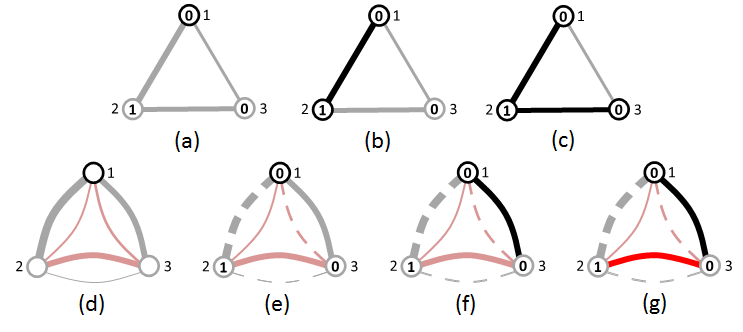
\includegraphics[width=3.3in]{AMWCS}
\caption{(a) to (c) and (d) to (g) show the construction of  one-edge AMWCS and two-edge AMWCS, respectively. The value in each node represents the allele. The width of each edge corresponds to the strength of dependency measure between pairs. For (d) to (g), the gray and black edges represent the L(00$\cup$11) edge, while the pink and red edges represent the L(00$\cup$11) edge. Nodes and edges with color black or red represent the determined AMWCS.}
\end{figure}


Figure 2 depicts different results of model construction with  a problem of three bits, and a receiver with alleles \{0, 1, 0\}. First, the node 1 with allele 0 was randomly chosen from the candidate set \{1, 2, 3\}. For the one-edge scheme in Figure 2(b), node 3 is selected with the strongest edge \{1, 2\}. After two iterations, the inserted node sequence of the AMWCS  is $Q = \langle\{1, 2, 3\}\rangle$, and the ILS is  $=\langle\{1\}, \{1, 2\}, \{1, 2, 3\}\rangle$. For the two-edge scheme in Figure 2(d), although there is a strong gray edge between nodes 1 and 3,  the pattern 10 conflicts with the meaning of gray edges.  According to the linkage selection rule, the thin red edge $L(01\cup10)$ represents the linkage between nodes 1 and 3 with pattern 01. For clarity, we illustrate conflict edges with dotted lines. Same scenario happens to other edges in Figure 2(e). Unlike the one-edge scheme, node 3, with the strongest solid edge \{1, 3\}, is picked in Figure 2(f). Therefore, the inserted node sequence of the AMWCS is $Q = \langle\{1, 3, 2\}\rangle$,  and  ILS is  = $\langle\{1\}, \{1, 3\}, \{1, 3, 2\}\rangle$.

Consider an instance with  optimal subsolution 111 with  strong  linkage among these three bits. Following the procedures described above, the one-edge graph constructs the ILS as $\langle\{1\}, \{1, 2\}, \{1, 2, 3\}\rangle$. However, None of mask in the ILS can flip the receiver with pattern 001 to 111. In short, even if one-edge graphical linkage model detects the correct model, it might still fail during mixing since the pattern might not be the optimal subsolution.


On the other hand, two-edge graphical linkage model  handles this problem by taking the alleles of receivers into account and preserve the correct pattern during mixing. We believe that the ratio of a pattern in the population corresponds to the possibility of such pattern being the optimal subsolution. The two-edge model tends to align the alleles of receiver  with the dominant patterns in the population. The reason for such tendency lies in the characteristic of mutual information. Since the mutual information between two bits is divided into two parts in the two-edge graph,  the  linkage containing the high-ratio pattern  is often positive, while the other part is usually negative.  In the example above, if the optimal subsolution 111 is prominent in the population, then the linkages $L(00\cup11)$ among these nodes should be positive, and the linkages $L(01\cup10)$ are likely negative.  In Figure 2(d), the two-edge graph starts with node 1, and the receiver has pattern  001. Unlike the one-edge model, the ILS  $\langle\{1\}, \{1, 3\}, \{1, 3, 2\}\rangle$ is only constructed with solid edges. For the two-edge scheme, choosing the mask \{1, 3\} can help flipping the pattern 001 to the the optimal subsolution 111.    


\begin{table}[ht]
\begin{tabular}{|c|c|c|c|c|}
\hline
 &
\multicolumn{2}{c|}{Supply length} &
\multicolumn{2}{c|}{Failure NFE in BM} \\
\hline
Problems  & One-edge & Two-edge & One-edge & Two-edge \\\hline
NK-S1 & 12.6 & 6.9  &51.3 & 43.4 \\\hline
NK-S3 & 13.2 & 6.9  &48.8 & 42.3 \\\hline
NK-S5 & 6.7 &2.6  & 10.1 & 8.9 \\\hline

\end{tabular}
\caption{Supply length and BM failure comparison}
\end{table}


\subsection{Supply bound}
Although taking the receivers into account enhance the effectiveness of bit-flipping, we find the two-edge scheme costs more evaluations in the mixing stage, especially during back mixing. The reason behind this phenomenon is supply overfitting. After selecting an edge in the two-edge graph, only the complement patterns are taken into account. For each pair of bits, the possible patterns are narrowed down to either \{00, 11\} or \{01, 10\}. Besides, we choose the node that gives the maximum linkage during model construction, meaning that the two selected patterns should have higher ratio in the population. Therefore, given a model constructed by a two-edge graph implies a higher possibility of finding the complement pattern in the population. This gives the models that are customized for a specific receiver a greater chance to pass the supply check. Figures 1(a) and 1(c) demonstrate the model construction with one-edge graph and two-edge graph for a receiver 010 starting with node 1. In the second iteration, picking node 3 instead of node 2 implies the ratio of patterns \{00, 11\} between nodes 1 and 3 is higher than the ratio of patterns \{01,10\} between nodes 1 and 2. Compared to the model constructed by one-edge graph in Figure 1(a), the model in Figure 1(c) is more likely to pass the supply check since the complement pattern has a higher ratio in the population. 

The customized model is effective in restricted mixing, but when the receiver becomes the donor in back mixing, this model is considered to be overfitting the donor. The experiment results in Table 2 show that the average supply bound of the two-edge graph is about two times longer than the one-edge counterpart. Normally, the supply bound prohibits recombination of longer patterns. However, when using the supply bound that is overfitting the donor in back mixing, it is likely to try more patterns or even copy the complete chromosome to each receiver in the population. This increase failure attempts and also the probability of cross competition in back mixing. 

To avoid overfitting supply bound, we adopt the one-edge graph for the supply bound. The major difference is that the linkage measure in the one-edge graph is calculated with complete mutual information, which represents the global information of population. On the other hand, the linkage measure in the two-edge graph is more skewed that favors the given receiver during model building. Therefore, using the supply bound of the one-edge graph secures the global information between bits and does not over fit a specific chromosome. This gives a better result in back mixing and reduce NFE.


Furthermore, we also find the one-edge graph supply bound benefits restricted mixing by enhancing the success rate of recombination. We speculate that in the early generations, subproblem patterns with better fitness do not stand out from the average patterns. The dependency information in the population is rather unclear. The inaccurate models then increase the probability of failure for restricted mixing. However, the restricted mixing operator only terminates if the fitness of receiver improves or the supply bound is reached. With the smaller masks bounded by the one-edge graph supply bound, unnecessary recombination trials are reduced during restricted mixing. 


\begin{algorithm}
\caption{Modified Restricted Mixing}\label{algo_disjdecomp}

$V$: candidate vertices set, $V_S$: $AMWCS$ vertices set,  \\
$ILS$: incremental linkage set, $f$: evaluation function, \\
$P$: population, $l$: problem size, \\
$T$: trial solution, $M$: mask, \\
${R_M}$: pattern of $R$ extracted by $M$, \\
${R_M}'$: complement pattern of ${R_M}$

\SetKwInOut{Input}{input}\SetKwInOut{Output}{output}
\Input{ $R$: receiver }
\Output{ $R$: reciever, $M$: mask }

\BlankLine
%\tcp{ construct ILS }
$V \leftarrow \{ 1, 2, ..., l \}$ \\
%$V_S \leftarrow \{v$ | a random vertex $v \in V \}$ \\
$V_s \leftarrow$ a random vertex $v \in V$ \\
remove $v$ from $V$ \\

\While{$ |V| \geq l/2$} {

    $ILS \leftarrow ILS \cup V_{S}$ \\
    $V_S \leftarrow V_S$ $\cup$ \{ the nearest vertex $v \in V \}$ \\
    %add the nearest vertex $v \in V$ into $AMWCS$ \\
    remove $v$ from $V$ \\
}

\BlankLine
\For{$i \leftarrow 1$ \KwTo $|ILS|$} {

    $M \leftarrow ILS_i$ \\

    \If {${R_M}' \subset P$} {

        $T \leftarrow R$ \\
        $T_M \leftarrow {R_M}'$ \\

        \If {$T \in P$} {
            \Return ($R$, $\emptyset$) 
        }

        \If {$f(T) \geq f(R)$} {
            $R \leftarrow T$ \\
            \Return ($R$, $M$)
        }
    }
}
\Return ($R$, $\emptyset$) 
\end{algorithm}

\subsection{Chromosome Existence Check}
%Break prevents possible cross over and limit attempts for useless function call. 
%Demo by table, showing how many attempt is useless after isInP and how often does cross competition occur
%If a mask failed the supply check, all masks with larger size behind it in the ordered ILS are discarded.

We propose a new termination criterion for restricted mixing that reduce the probability of cross-competition. During restricted mixing, the masks in the ILS are tried in an ascending order regarding to the mask size. Occasionally, the recombination creates a chromosome that has already exists in the population. If the new pattern gives worse fitness value than the original one, the receiver continues to try bit-flipping with the next larger mask. This bit-flipping process only terminates if the fitness of the generated chromosome is not inferior to the fitness of the original receiver. We find this termination criterion easily leads to cross-competition since there is a great chance to try larger masks that includes two subproblems. If one of the subproblem pattern is not the optimal pattern, it might lead the population to converge to the wrong pattern after back mixing.

For example, consider a six-bit problem with two deceptive three-bit traps. The two subproblems have the same optimal pattern 111 and a second best pattern 000. Suppose the pattern 000000 already exists in the population. Without loss of generality, consider performing restricted mixing on a receiver 111000 with a ILS = $\langle\{1\};\{1,3\}, \{1,3,2\}, ...,\\ \{1,3,2,4,6,5\}\rangle$. Mask \{1\} and \{1,3\} leads to failure recombination since 011 and 010 have fitness less than pattern 111. After trying the third mask \{1,3,2\} on receiver 111000, the resulting chromosome 000000 already exists in the population. However, the restricted mixing process continues due to the inferior fitness of pattern 000000 compared to the fitness of receiver 111000, which contains one suboptimal. Mask \{1,3,2,4\} and \{1,3,2,4,6\} also leads to failure recombination. Finally, with the mask \{1,3,2,4,6,5\}, a chromosome 000111, which has equal fitness as the receiver 111000, is generated. This recombination is accepted and the receiver becomes the donor in back mixing that tries pattern 000111 on all the other chromosomes in the population. The pattern 000111 is the second best solution that is able to replace all patterns except for 111000 under the strict-improvement criterion of back mixing. If 111000 does not exist in the population, the algorithm failed with the first three bits of the population converged to the wrong pattern 000.  Even if 111000 exists in the population, the population might have already converged to only two patterns, 111000 and 000111. Then the back mixing operator switch to the equal-acceptance criterion and the algorithm failed with the population converged to the wrong pattern 000111.


To prevent this situation, we terminate restricted mixing whenever the new generated chromosome already exists in the population. Another receiver along with another set of customized models are chosen for the next iteration of restricted mixing. This criterion decreases the probability of ruining optimum and reduces occurrence of cross-competition. The pseudocode of the modified restricted mixing is given in Algorithm 4.








\section{EXPERIMENT RESULTS}
In this section, we first briefly introduce the six benchmark problems. After that, the experiment setup is given. Finally, we illustrate the experiment results of the original DSMGA-II, the improved DSMGA-II, LT-GOMEA and hBOA. 


\subsection{Test Problems}
 Six types of linkage benchmark problems are used in this paper, including four classical linkage-underlying problems and two real-world problems. These benchmark problems each covers different aspects and characteristics of real-world problems. The Concatenated Trap is composed of m additively separable trap functions, each with k variables [8]. It is well known that in order to solve trap problems, the underlying structure must be detected and preserved during mixing [9]. The Cyclic Trap consists of overlapping trap functions with wraparound [10]. The Folded trap is one of the multiple variants of NK-landscape problems described in [11]. We use the bipolar deceptive function with the subsolution size k = 6. Each subsolution contains two global optima and lots of local optima. It The performance depends heavily on the ability of reducing unnecessary exploration of plateaus due to the symmetric characteristics of the trap function. The NK-landscape functions are composed of overlapped and randomly generated sub-functions [12]. Each instance is controlled by three parameters: the problem size l, the number of neighbors of one gene k, and the step size s, i.e. the offset of two adjacent sub-functions. We use NK-landscape with step 1, 3 and 5 to represent problems with different degrees of overlapping in our experiments. The Ising spin-glass gives a set of variables in one of the two states {+1, -1}. For each pair of neighboring spins i and j, there exists a coupling constant Jij. The goal is to find a combination of states that satisfies the most coupling pairs. The Maximum Satisfiability problem (MAX-SAT) consists of a series of logical and clauses. Each clause contains a series of logical or variables. It is a classical NP-complete problem.  


\subsubsection{Concatenated trap}


\begin{displaymath}
f_{m,k}^{trap}(x) = \sum_{i=1}^{m} f_{k}^{trap} \left (\sum_{j = i\cdot k-k+1}^{i\cdot k} x_j\right )
\end{displaymath}

where

\begin{displaymath}
f_{k}^{trap}(u) = 
   \begin{cases}
    1, & \text{if $u=k$} \\
    \frac{k-1-u}{k}, & \text{otherwise}
	\end{cases}
\end{displaymath}




\subsubsection{Cyclic trap}


\begin{displaymath}
f_{m,k}^{cyclic}(x) = \sum_{i=1}^{m} f_{k}^{trap} \left (\sum_{j = i\cdot(k-1)-k+2}^{i\cdot(k-1)+1} x_j\right )
\end{displaymath}

where

\begin{displaymath}
f_{k}^{trap}(u) = 
   \begin{cases}
    1, & \text{if $u=k$} \\
    \frac{k-1-u}{k}, & \text{otherwise}
	\end{cases}
\end{displaymath}

and

\begin{displaymath}
x_j = x_{j-l}, \text{if } l < j \leq 2l
\end{displaymath}




\subsubsection{Folded trap}



\begin{displaymath}
f_{m,k=6}^{folded}(x) = \sum_{i=1}^{m} f_{k=6}^{folded} \left (\sum_{j = i\cdot k-k+1}^{i\cdot k} x_j\right )
\end{displaymath}

where

\begin{displaymath}
f_{k=6}^{folded}(u) = 
   \begin{cases}
    1, 		& \text{if $|u=3| = 3$} \\
    0.8, 	& \text{if $|u=3| = 0$} \\
    0.4, 	& \text{if $|u=3| = 1$} \\
    0, 		& \text{if $|u=3| = 2$} \\
	\end{cases}
\end{displaymath}


\subsubsection{NK-landscape}

\begin{displaymath}
f_{l,k,s}^{NK}(x) = \sum_{i=0}^{(l-k-1)/s} f_{k,i}^{subNK} (x_{i{\cdot}s+1},x_{i{\cdot}s+2},...x_{i{\cdot}s+k+1})
\end{displaymath}


\subsubsection{Ising spin-glass}

\begin{displaymath}
f_{n}^{spin}(x) = -\sum_{i,j=0}^{n} x_{i}x_{j}J_{ij}
\end{displaymath}

\subsubsection{MAX-SAT}

\begin{displaymath}
F = \bigwedge_{i=1}^{m} \left (\bigvee_{j=1}^{k_{i}} l_{ij} \right )
\end{displaymath}


\subsection{Experiment Setup}
DSMGA-II is an enhanced edition of DSMGA and it outperforms multiple variants of its predecesor~\cite{yu:DSMGA} in all cases. 
Thus, we shall not discuss DSMGA in the following comparison.
DSMGA-II is based on the idea of OM, so it is necessary to compare DSMGA-II with GOMEAs. 
In our comparison, LT-GOMEA with forced improvement \footnote{http://homepages.cwi.nl/$\sim$bosman/source\_code.php} is used as a benchmark GOMEA algorithm.
Although several different linkage models have been proposed over the years~\cite{bosman:robust}, LT-GOMEA~\cite{bosman:LT-GOMEA} is still considered a state-of-the-art OM algorithm.
Also, we compare DSMGA-II with the hierarchical Bayesian optimization algorithm (hBOA)~\cite{pelikan:hBOA}
Similar to LT-GOMEA, hBOA is also a milestone that is often used in recent EDA researches.


A minimum population is required for a certain number of consecutive successful runs.
However, the conventional bisection procedure~\cite{pelikan:hBOA} often failed to yield the minimum NFE, since the minimum population size varies in the bisection procedure for different algorithms.
In the following experiments, we adopt an adaptive sweeping procedure for more accurate search of minimum NFE.
The sweeping procedure starts with a reasonalbe population size.
The initial population size is set as 10 in this paper.
If the algorthm cannot consecutively reach the global optimum with the given population, the population size is increased with a predefined step.
In this paper, the initial step is set to be 30, and 10 back-to-back successful hits is defined as a successful trial.
The mean of NFE over 10 successful runs is recorded as the minimum NFE required for a given population size.
After a successful NFE is recorded, a smaller step is adopted to narrow down the sweeping range.
The sweeping procedure continues until the step converges.
In this paper, we divide the step by 2 for each iteration, and the procedure terminates if the sweeping range is within 5\% of the population size.
The sweeping procedure gives better precision than the canonical bisection procedure, since the acquired resolution increases as the steps decreases after each successful trial.
The resulting minimum NFE for each problem is averaged over 100 independent runs or instances.

We compare DSMGA-II, LT-GOMEA, and hBOA under the following settings. The selection pressure is set as 2 for all three algorithms. 
For DSMGA-II, the model building is performed every $\ell/50$ generations.
LT-GOMEA is performed without local searh to enhance its performance, described in~cite{}.




\subsection{Results}

\subsubsection{ Comparison with the original DSMGA-II }

\begin{table}[ht]
\centering
\begin{tabular}{ |c|c|c|c| } \hline
\textbf{Problems}& \textbf{Original} & \textbf{Improved} & \textbf{Ratio}\\ \hline
\textbf{Cyclic trap}, $\ell = 400$ 		& 123.1&111.5&9.4\%\\ \hline
\textbf{Folded trap}, $\ell = 480$	 	& 354.5& 243.2&31.4\%\\ \hline
\textbf{NK-S1}, $\ell = 400$ 				& 767.4& 701.6&8.5\%\\ \hline
\textbf{NK-S3}, $\ell = 400$ 				& 550.5& 533.5&3.1\%\\ \hline
\textbf{NK-S5}, $\ell = 400$ 				& 62.0& 59.5&4.1\%\\ \hline
\textbf{Ising spin-glass}, $\ell = 784$ 	& 863.2&684.5&20.7\%\\ \hline
\textbf{MAX-SAT}, $\ell = 200$ 			& 7593.3& 5655.1&25.5\%\\ \hline
\end{tabular}
\caption{Required NFE of DSMGA-II for the largest test problems}
\end{table}

Comparing with the original DSMGA-II, our new techniques show superior performance on all six benchmark problems.
In Table 2, comparison between our new techniques along with the original DSMGA-II are shown only with the largest problem size since the improvement is relatively minor with smaller problems. 
The results indicate that our new techniques can reduce NFE up to 30\% compared to the original DSMGA-II. 


Our new technique is most effective when dealing with folded trap problems.
The two-edge AMWCS is capable of constructing customized models for a chosen receiver. 
This characteristic shows great advantage when facing problems with multiple equal-quality subsolution, such as folded trap problems.
Since the two-edge model tends to align with the most promenant pattern in the population, it cost less NFE to jump out of plateaus by converging through stronger drifting effect.


This characteristic is also helpful with solving Ising spin-glass problems. 
There are often two equal-fitness subsolutions in the spin-glass problem.
The original DSMGA-II can only detect the strong linkage of the subsolution without knowing the correct pattern of the subsolution to contribute to global fitness.
This results in a notable waste of NFE when repeatedly flipping subsolution patterns to another equally fit subsolution during mixing.
With the two-edge AMWCS, different models can be generated with the same linkage graph. 
Empirically, this helps preserve the optimal patterns during mixing and reduce attempts of trying the complementary pattern.


The improved DSMGA-II requires less NFE than both LT-GOMEA and hBOA on all six benchmark problems.
It is worth mentioning that most of the slope of DSMGA-II data line decreases as the problem size increases.
This indicates that the improved DSMGA-II excels in scalability.
The following parts divides the six benchmark problems in three categories according to their characteristics. 


\begin{figure}
\centering
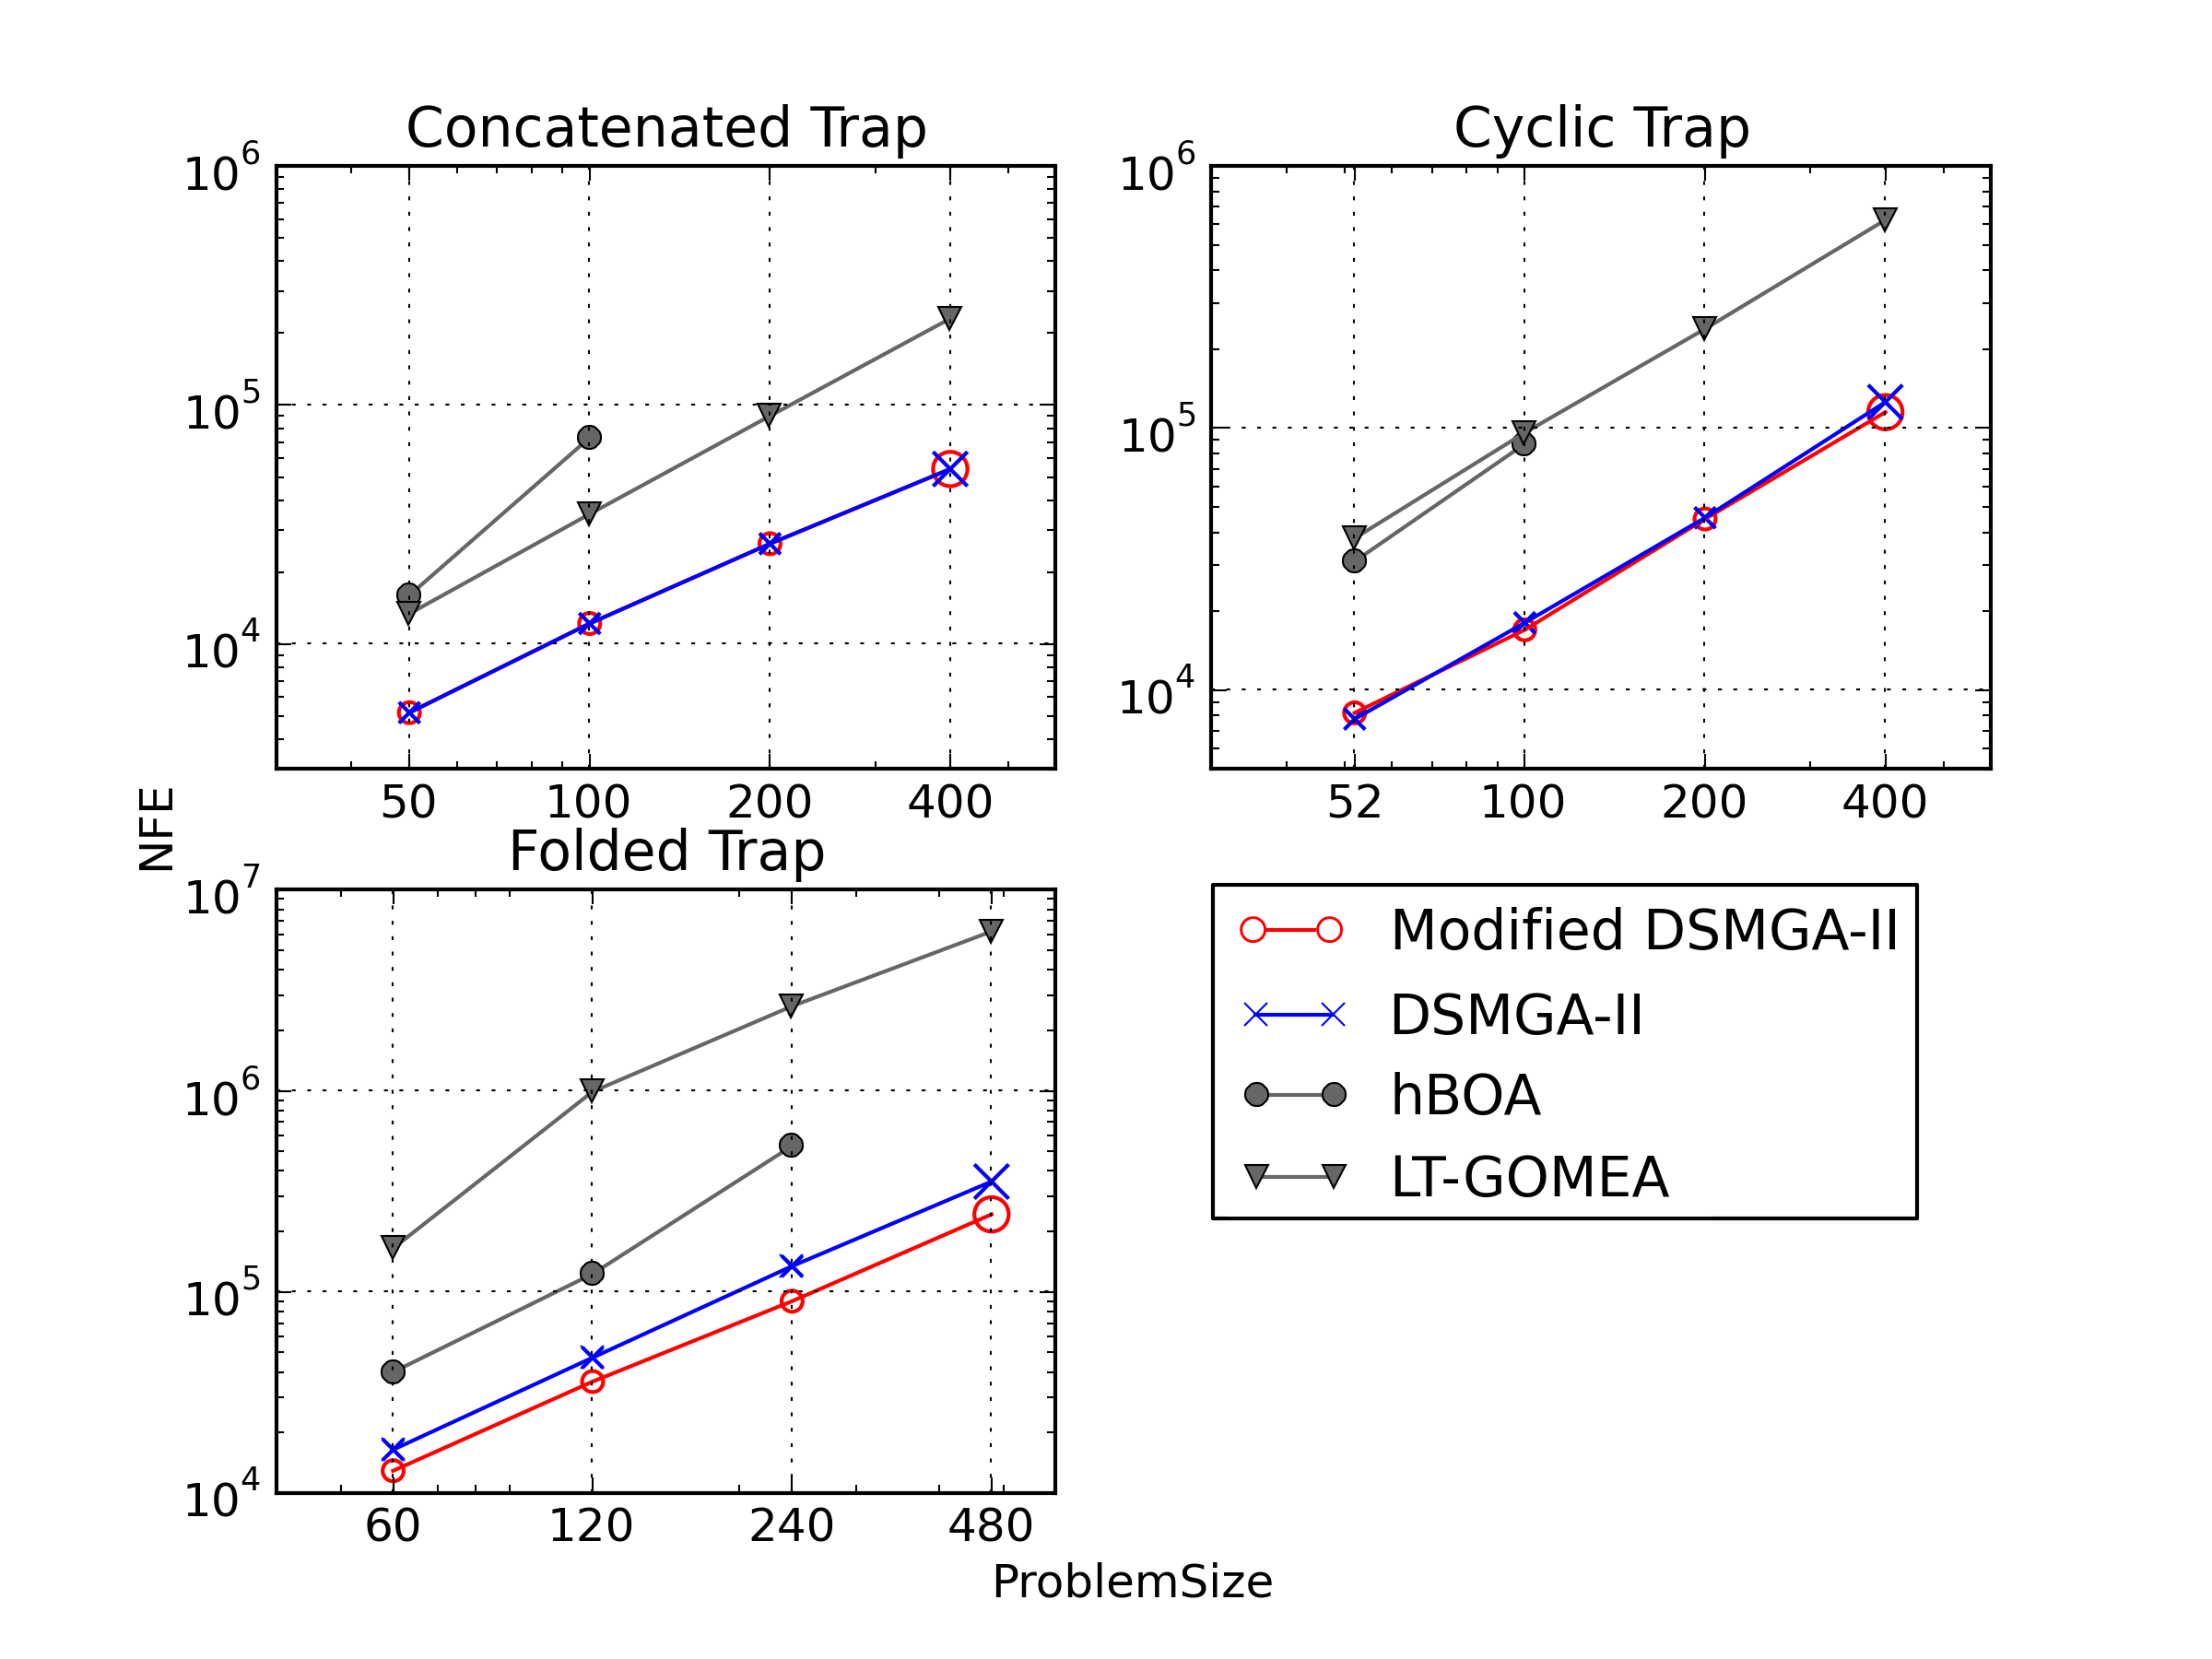
\includegraphics[width=3.3in]{trapResults}
\caption{Scalability of DSMGA-II, LT-GOMEA and hBOA on the problems of deceptive variants.}
\end{figure}

\subsubsection{ Comparison on deceptive variants }


We first consider the deceptive problems in Figure 2.
For concatenated trap problems, DSMGA-II requires less NFE than LT-GOMEA and hBOA.
For folded trap problems, the two-edge model helps aligned the receiver with the promenant pattern in population.
Together with back mixing, the pattern soon dominates the population, and the population is able to jump out of the plateau. 
This strong and precise drifting effects is the key to the outstanding performance of DSMGA-II on folded trap problems.


For cyclic trap, most of patterns converges to three, four or five consecutive 1s or 0s after local search.
Afterwards, it is crutial to construct a model that contains all zeros in order to be flipped to all ones. 
The original AMWCS can only detect the subproblem structures, but the two-edge AMWCS can further construct a most suitable structure for a specific receiver. 
For instance, consider a chromosome 111100000 with its AMWCS starting from 5-th bit with allele 0.
Both the one-edge and two-edge AMWCS detects a strong linkage between the four bits on the left and the four bits on the right.
For the one-edge model, there is a fifty-fifty chance to choose a bit from the first four bits or the last four bits to add into the AMWCS. 
However, if one of the first four bits is chosen as the second node of AMWCS, all mixing attempts shall fail since flipping 11110 to 00001 results in worse fitness.
To make matters even worse, cross-competition might occur if 111100000 is flipped to 000011111. 
This pattern might dominate the population in back mixing by converging all first four bits to zeros.
With the two-edge model, the linkages $L(01\cup10)$ between the 5-th bit and first four bits are going to be negative. 
The all 1s and all 0s patterns helps enhance the $L(00\cup11)$ linkage in the two-edge AMWCS graph.
As a result, the second node must be selected from the last four bits, which has the same allele 0 as the 5-th bit.
Once the model 00000 is selected during mixing, the 111100000 can be flipped to global optimum.


\subsubsection{ Comparison on NK-landscape problems }

\begin{figure}
\centering
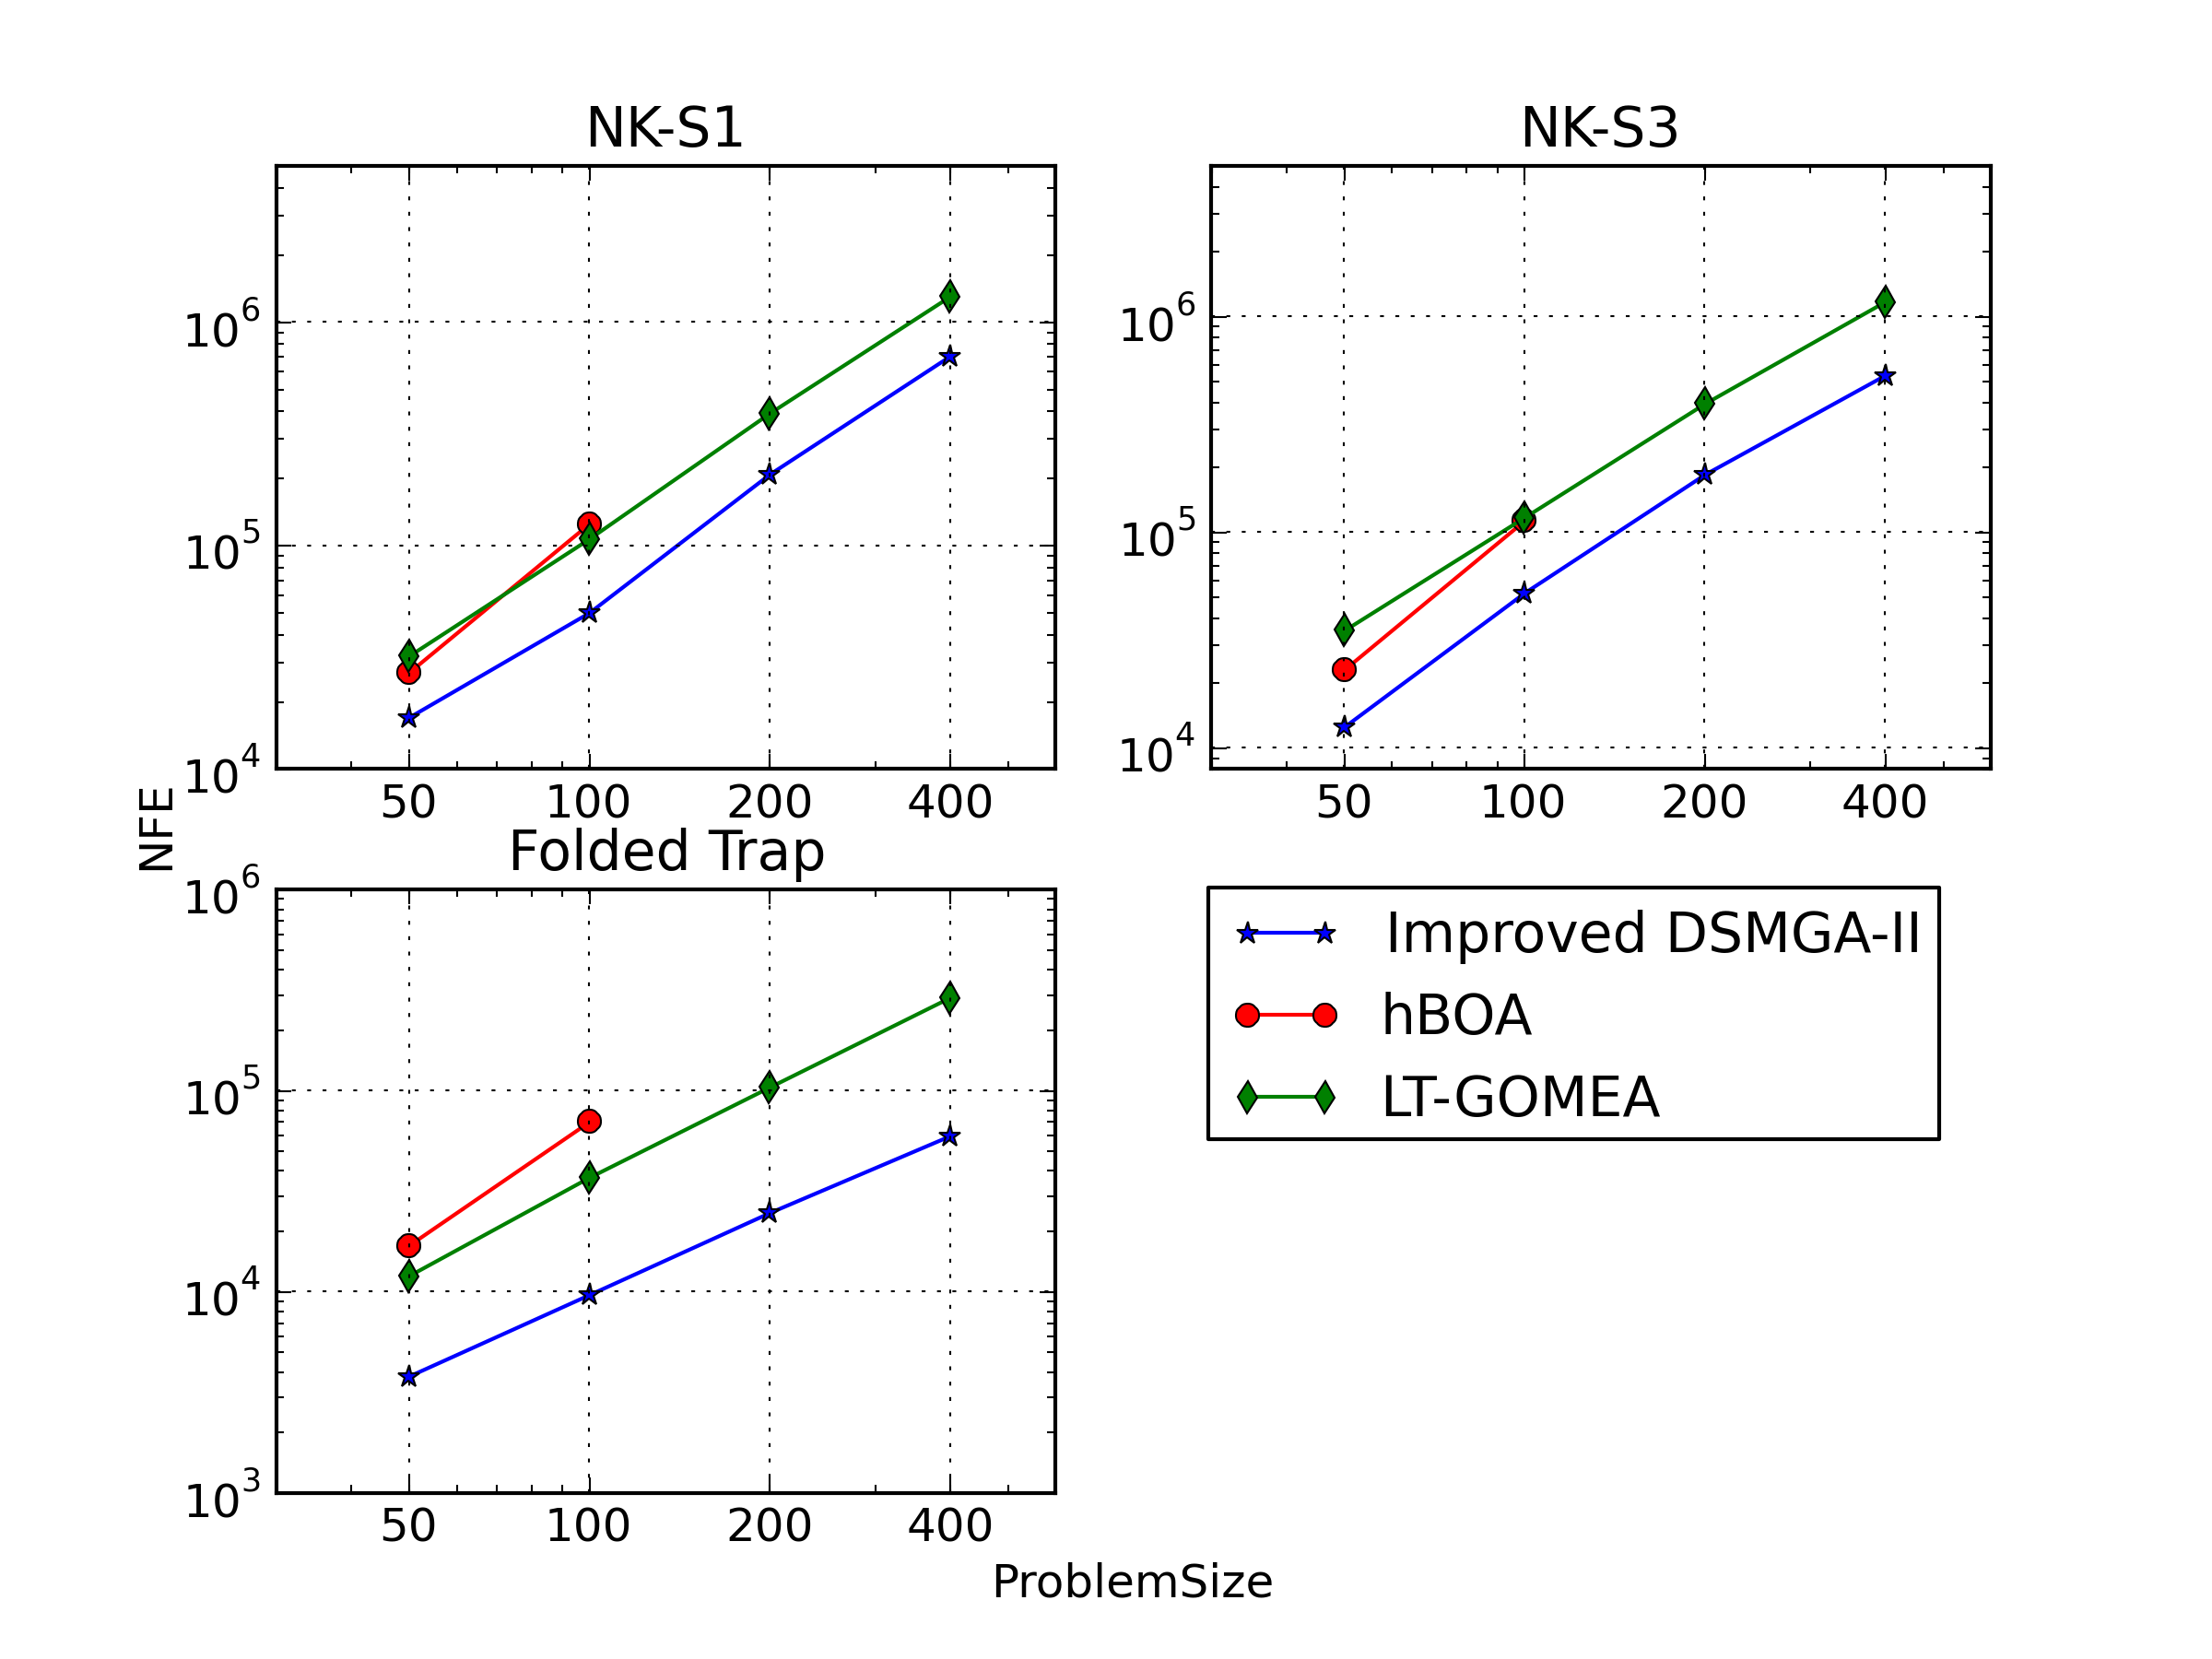
\includegraphics[width=3.3in]{nkResults}
\caption{Scalability of DSMGA-II, LT-GOMEA and hBOA on NK-landscape problems with various degrees of overlapping.}
\end{figure}


The NK series in Figure 2.
The result shows the ability of the ILS model in handling randomly generated overlapping problems. 
The difference between DSMGA-II and other algorithms enlarges as the degree of overlapping decreases. 
When coping with severly overlapped structures, DSMGA-II requires more NFE during graph refining process.
Once the linkage information stands out, the back mixing operator allows the correct pattern to dominate the population instantly 
The two-edge model provides far more linkage combinations in solution space.
Generating ILS from the abundant combinations in the two-edge AMWCS results in more flexible and better customized models.
These models enable DSMGA-II to handle overlapping problems nicely. 


\subsubsection{ Comparison on real-world problems }



For results of Ising spin-glass problems in Figure 6, the slope of DSMGA-II decreases as the problem size increases. 
This is due to the numerous numbers of plateaus in the spin-glass problems.
As discussed in Section 4.3.1, converging the population for plateaus is where the advantages of DSMGA-II holds.
Moreover, the slope indicates the overall fitness evaluation grows polynomially as $O(n^3)$, which is close to the best known results of problem-specific algorithm for Ising spin-glass~\cite{galluccio:pfaffian}

For MAX-SAT problems, although the NFE seems to grow exponentially, DSMGA-II still requires the fewest evalutions among the three algorithms.



\section{Conclusions}
This paper proposes a new two-edge graphical linkage model for DSMGA-II. 
Some new techniques are also adopted to constructs a more precise linkage model that gives building-blocks customized for each receiving chromosome during mixing.
We also show that early-stopping technique can reduce the probability of cross-competition, allowing DSMGA-II to solve the benchmark problems with a smaller population and less NFE.
The improved DSMGA-II decrease NFE by up to 20\% compared with the original version. It also outperforms LT-GOMEA and hBOA on multiple benchmark problems. 

\begin{figure}
\centering
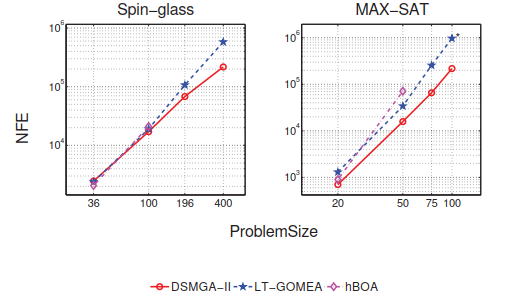
\includegraphics[width=3.3in]{spin_satResults}
\caption{Scalability of DSMGA-II, LT-GOMEA and hBOA on Spin-glass and MAX-SAT (*LT-GOMEA fails to reach the global optima for two instances with $\ell=100$ on MAX-SAT).}
\end{figure}
%\end{document}  % This is where a 'short' article might terminate

%ACKNOWLEDGMENTS are optional
%\section{Acknowledgments}
%The authors would like to thank the support by Ministry of Science and Technology in Taiwan under Grant No. MOST 103-2221-E-002-177-MY2-1.

%
% The following two commands are all you need in the
% initial runs of your .tex file to
% produce the bibliography for the citations in your paper.
\bibliographystyle{abbrv}
\bibliography{sigproc}  % sigproc.bib is the name of the Bibliography in this case
% You must have a proper ".bib" file
%  and remember to run:
% latex bibtex latex latex
% to resolve all references
%
% ACM needs 'a single self-contained file'!
%
%\balancecolumns % GM June 2007
% That's all folks!



\end{document}
